% -----------------------------------------------------------------------------
% ########################
% # PREDLOGA ZA POROCILO #
% ########################
%
% @author Iztok Starc
% @date   3. december 2008
%
\documentclass[a4paper,12pt]{report}

% -----------------------------------------------------------------------------
% ####################################################
% # UPORABA PAKETOV - NASTAVITEV JEZIKA in KODIRANJA #
% ####################################################
\usepackage[slovene]{babel}
\usepackage[utf8]{inputenc}
\usepackage{lmodern}
\usepackage[T1]{fontenc}
\usepackage[sc]{mathpazo}
\linespread{1.05}
\usepackage[T1]{fontenc}

% -----------------------------------------------------------------------------
% ######################################
% # VNOS KLJUCNIH PARAMETROV BESEDILA  #
% ######################################

\newcommand{\naslov}     {Spletna trgovina}
\newcommand{\prviavtor}  {Matic Novak}
\newcommand{\prviindeks} {63130164}
\newcommand{\drugiavtor} {Jakob Košir}
\newcommand{\drugiindeks}{63130115}
\newcommand{\kraj}       {Ljubljana}

% -----------------------------------------------------------------------------
% ###################
% # UPORABA PAKETOV #
% ###################
\usepackage[a4paper,left=25mm,right=25mm,top=20mm,bottom=30mm,includehead]{geometry}

\usepackage{graphicx, epsfig}

\usepackage{fancyhdr}

\usepackage[
colorlinks=true, linkcolor=blue, citecolor=red,
%
pdftitle={\naslov},
pdfauthor={\prviavtor, \drugiavtor},
pdfsubject={Poročilo seminarske naloge pri predmetu Elektronsko Poslovanje},
pdfkeywords={spletna prodajalna, PHP, SSL, MySQL}, a4paper, pagebackref=true, unicode]{hyperref}

% -----------------------------------------------------------------------------
\begin{document}

% -----------------------------------------------------------------------------
% ##################
% # NASLOVNA STRAN #
% ##################
\begin{titlepage}
	\begin{center}
	{UNIVERZA V LJUBLJANI\\[10pt] 
	FAKULTETA ZA RAČUNALNIŠTVO IN INFORMATIKO}

	\vspace{65mm}

	{\Large\textbf{\naslov}}

	\vspace{10mm}

	{\large Poročilo seminarske naloge pri predmetu\\[10pt] Elektronsko poslovanje}

	\vfill
	\vspace{60mm}

\hspace{20mm}
\begin{minipage}[t]{70mm}
	{\bf Študenti}\\
	{\prviavtor} ({\prviindeks})\\ 
	{\drugiavtor} ({\drugiindeks})\\
\end{minipage}
%\hfill
\begin{minipage}[t]{50mm}
	{\bf Mentor}\\
	David Jelenc
\end{minipage}
%\hspace{20mm}

	\vspace{35mm}

	{	\kraj, \today}
	\end{center}
\end{titlepage}

% -----------------------------------------------------------------------------
% ##################
% # KAZALO VSEBINE #
% ##################

\tableofcontents

% -----------------------------------------------------------------------------
% ############
% # POVZETEK #
% ############
%\begin{abstract}
%\end{abstract}

% -----------------------------------------------------------------------------
% ##################
% # UVOD DOKUMENTA #
% ##################
\chapter{Uvod}

V seminarski nalogi sva se osredotočila predvsem na varno programiranje. Strežniški del spletne trgovine sva razvila v programskem jeziku php, pogled pa v tehnologijah html, css in javascript. Razvila sva tudi Android aplikacijo, ki preko rest api-ja dostopa do izdelkov na strežniku in jih ustrezno prikaže na mobilni napravi.

% -----------------------------------------------------------------------------
% ###################
% # JEDRO DOKUMENTA #
% ###################

% -----------------------------------------------
\chapter{Navedba realiziranih storitev}

Implementirala sva vse razširjene storitve, ki se tičejo varnosti in uporabniškega vmesnika: vodenje dnevnika uporabnikov, registracija s captcho, potrditveni e-mail ob registraciji, uporabniški vmesnik s html-jem, css-om in ajax-om, ocenjevanje artiklov, iskanje po artiklih, slike artiklov.


% -----------------------------------------------
\chapter{Podatkovni model}

Podatkovni model sestavlja 8 tabel. Tabela Uporabnik hrani vse uporabnike, ki uporabljajo portal (administratorje, prodajalce in stranke). Da je model normaliziran, poštne številke in pošte hraniva v svoji tabeli. Tabela PrijavaLog služi za vodenje dnevnika uporabnikov. Tabela Izdelek hrani podatke o artiklih v trgovini. Vsak izmed njih ima lahko več slik in več ocen različnih uporabnikov, zato sta to še dve ločeni tabeli. V tabeli Narocilo hranimo vsa naročila, tabela PostavkaNarocila pa hrani vse postavke vseh narocil. Brez nje bi imeli povezavo "many to many" med naročili in izdelki, tako pa model ne bi bil normaliziran.\newline
Vse atribute se da smiselno interpretirati iz njihovih imen. Mogoče bi omenila zgolj gesla, ki se hranijo v tabeli Uporabnik. Pred zapisom v bazo se nad nizom kliče php funkcija password\_hash, ki geslo v več iteracijah izračunov spremeni v izvleček. Tako ne more priti do razkritij gesel, če nepooblaščeni osebi uspe pridi do baze.

\begin{figure}[htb]
	\centering
	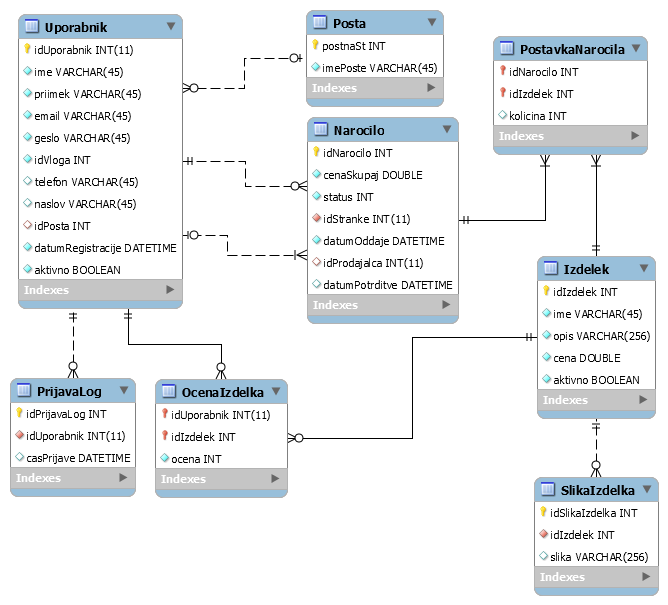
\includegraphics[width=13cm]{img/er-trgovina.png}
	\caption{ER diagram podatkovne baze}
\label{fig:1}
\end{figure}

% -----------------------------------------------
\chapter{Varnost sistema}

Opišite implementirane mehanizme za nadzor dostopa ter ostale kontrole, ki ste jih implementirali. Pri vsake navedite, kaj je njen namen oz. katere varnostne grožnje preprečuje.

Kot elementarni način za zagotavljanje pravilnosti podatkov izvajava validacijo vseh obrazcev z regularnimi izrazi. V primeru, da uporabnik ne zadosti zahtevam, se ga na to opozori, podatki pa se sploh ne pošljejo na strežnik. Seveda se da podatke poslati na strežnik tudi mimo obrazcev, zato prejete podatke še enkrat validirava na strani strežnika.

Vse prejete podatke najprej prečistiva z vgrajenimi php funkcijami in s tem preprečiva SQL INJECTION in XSS napade:\newline
($filter\_input(INPUT\_POST, data, FILTER\_SANITIZE\_SPECIAL\_CHARS$)

Dodatno poskrbiva za varnost pri registraciji uporabnika, saj mora pravilno prepisati znake s CAPTCHE. Preprečiva, da bi registracijo opravljal nek zlonamerni program.

Prodajalec in Administrator sta posebni vlogi v spletni trgovini, ki imata nadzor nad zaupnimi podatki. Za prijavo v omenjenih vloga zahtevava, da se uporabnik predstavi z ustreznim (veljavnim) certifikatom X.509.

% -----------------------------------------------
\chapter{Izjava o avtorstvu seminarske naloge}

Spodaj podpisani \textit{\prviavtor}, vpisna številka \textit{\prviindeks}, sem (so)avtor seminarske naloge z naslovom \textit{\naslov}. S svojim podpisom zagotavljam, da sem izdelal ali bil soudeležen pri izdelavi naslednjih sklopov seminarske naloge:
\begin{itemize}
	\item izdelava certifikatov in programske logike za prijavo z njimi
	\item preusmeritev na zavarovani kanal (HTTPS)
    \item prijava in odjava v/iz sistem(a)
    \item registracija uporabnika s CAPTCHO
    \item pošiljanje potrditvenega e-maila
    \item vodenje dnevnika uporabnikov
	\item urejanje uporabniških podatkov
	\item upravljanje s prodajalci in strankami
	\item izdelava rest storitve za izdelke
	\item izdelava Android aplikacije
	 
	 
\end{itemize}

Podpis: {\prviavtor}, l.r.

\newpage

Spodaj podpisana \textit{\drugiavtor}, vpisna številka \textit{\drugiindeks}, sem (so)avtor seminarske naloge z naslovom \textit{\naslov}. S svojim podpisom zagotavljam, da sem izdelal ali bil soudeležen pri izdelavi naslednjih sklopov seminarske naloge:
\begin{itemize}
	\item celotno upravljanje z izdeki
	\item ocenjevanje izdelkov
	\item iskanje po izdelkih
	\item predstavitev artiklov s slikami
    \item košarica z Ajax-om
	\item celotno upravljanje z naročili
\end{itemize}

Podpis: {\drugiavtor}, l.r.

\newpage

% -----------------------------------------------------------------------------
% #######################
% # ZAKLJUCEK DOKUMENTA #
% #######################
\chapter{Zaključek}

Seminarska naloga nama je bila všeč, predvsem zato, ker je bil tokrat povdarek na varnosti aplikacije in ne samo na njenih funkcionalnostih. Zavedava se, kaj vse se lahko zgodi s podatki, če ne poskrbimo za ustrezno varnost in težo posledic. Prvič sva implementirala prijavo s spletnimi certifikati, kar štejeva kot zelo uporabno znanje. 

% -----------------------------------------------------------------------------
% ##############
% # LITERATURA #
% ##############
\begin{thebibliography}{99}
\addtocounter{chapter}{1}
\addcontentsline{toc}{chapter}{\protect\numberline{\thechapter}Literatura}
\addtocontents{toc}{\protect\vspace{15pt}}

\bibitem{bib:ref} Yank K. \emph{Build Your Own Database-Driven Website Using PHP \& MySQL}. SitePoint, 2003. ISBN-10: 0-957-92181-0.

\bibitem{bib:ref1} Michele D.; Jon P. \emph{Learning PHP and MySQL}. O'Rielly, 2006. ISBN-10: 0-596-10110-4.

\bibitem{bib:ref2} Tim C.; Joyce P.; Clark M. \emph{PHP5 and MySQL Bible}. Wiley Publishing, Inc., 2004. ISBN-10: 0-7645-5746-7

\bibitem{bib:LinuxCommandReference} Red Hat Software inc. \emph{Linux Complete Command Reference}. Sams Publishing, 1997. ISBN-10: 0-672-31104-6.

\bibitem{bib:IPsecHowTo1} Ralf Spennberg. \emph{IPsec HOWTO} (online). 2003. (citirano \today). Dostopno na naslovu:
\url{http://www.ipsec-howto.org/t1.html}

\end{thebibliography}

\end{document}
